\begin{frame}{What Changes for Medical Images}
  \begin{columns}[T,onlytextwidth]
    \column{0.52\textwidth}
      \begin{itemize}\footnotesize\itemsep0.35em
        \item \textbf{Calibrated 3D data.} Computed tomography (CT) stores X-ray attenuation in Hounsfield units (HU: water 0, air $-1000$). Pipelines first clip HU to a window, level $\pm$ width/2, and rescale it (a soft-tissue window: width 400, level 40). CT and magnetic resonance imaging (MRI) arrive as stacks of slices, and models work on 3D patches.
        \item \textbf{Gigapixel pathology.} A whole-slide image (WSI) of stained tissue ``may comprise tens of thousands of image tiles'' (Xu et al., 2024).
        \item \textbf{Expensive labels.} One 3D CT lesion mask drawn by hand took 525.9\,s on average in the MedSAM2 annotation study.
        \item \textbf{Scanner shift.} In the fastMRI 2020 challenge, a data-format difference on an unseen vendor's scanner ``rendered many models useless in this track without modification''.
      \end{itemize}
    \column{0.46\textwidth}
      \centering
      {\scriptsize
      \begin{tabular}{@{}>{\raggedright\arraybackslash}p{1.3cm} >{\raggedright\arraybackslash}p{4.4cm}@{}}
        \toprule
        \textbf{Modality} & \textbf{What a pixel or voxel holds} \\
        \midrule
        CT & attenuation in HU; 3D volume \\
        MRI & sequence-dependent signal (T1- or T2-weighted) with no absolute scale; 3D volume \\
        X-ray & projected attenuation; 2D \\
        Ultrasound & acoustic echoes; 2D video \\
        WSI & colour of tissue stained with haematoxylin and eosin (H\&E); gigapixel 2D \\
        \bottomrule
      \end{tabular}\par}
      \vspace{0.5em}
      \begin{tcolorbox}[colframe=KAred, colback=gray!6, boxrule=0.5pt, left=4pt, right=4pt, top=3pt, bottom=3pt]
        \footnotesize \textbf{Dice coefficient}, the default overlap score:
        \[ \mathrm{Dice}(P,G) = \frac{2\,|P \cap G|}{|P| + |G|} \]
        $P$: predicted voxels; $G$: reference voxels. 1 is perfect overlap, 0 is none.
      \end{tcolorbox}
  \end{columns}
  {\scriptsize Ma et al., Nature Communications 2024, \href{https://arxiv.org/abs/2304.12306v3}{arXiv:2304.12306v3}, Methods; Xu et al., Nature 2024; Ma et al., \href{https://arxiv.org/abs/2504.03600v1}{arXiv:2504.03600v1}, Figure~3b; Muckley et al., \href{https://arxiv.org/abs/2012.06318v3}{arXiv:2012.06318v3}, Section~IV-A.\par}
\end{frame}

\begin{frame}{nnU-Net: Configure the Pipeline, Keep the U-Net}
  \begin{columns}[T,onlytextwidth]
    \column{0.40\textwidth}
      \centering
      \begin{tikzpicture}[font=\sffamily\scriptsize, >=latex,
          box/.style={draw, rounded corners=0.1cm, align=left, text width=4.6cm, inner sep=3pt},
          fpbox/.style={box, fill=cyan!15}, rulebox/.style={box, fill=yellow!25},
          trainbox/.style={box, fill=green!18}, pickbox/.style={box, fill=orange!16}]
        \node[fpbox, anchor=north] (fp) at (0,0) {\textbf{Dataset fingerprint}: image sizes, voxel spacings, modality, intensity statistics};
        \node[rulebox, anchor=north] (rules) at ($(fp.south)+(0,-0.32)$) {\textbf{Rules} plus the GPU budget set resampling, normalisation, patch size, batch size, topology; a fixed \textbf{blueprint} sets loss, optimiser, schedule, augmentation};
        \node[trainbox, anchor=north] (cv) at ($(rules.south)+(0,-0.32)$) {Train 2D, 3D full-resolution and 3D cascade U-Nets with 5-fold cross-validation};
        \node[pickbox, anchor=north] (pick) at ($(cv.south)+(0,-0.32)$) {\textbf{Empirical}: keep the best configuration or ensemble; post-process only if it helps};
        \draw[->] (fp) -- (rules);
        \draw[->] (rules) -- (cv);
        \draw[->] (cv) -- (pick);
      \end{tikzpicture}\\[0.3em]
      {\scriptsize Redrawn after Isensee et al., \href{https://arxiv.org/abs/1904.08128v2}{arXiv:1904.08128v2}, Figure~2b.\par}
    \column{0.58\textwidth}
      \begin{itemize}\scriptsize\itemsep0.25em
        \item \textbf{nnU-Net} (Isensee et al., Nature Methods 2021) keeps the U-Net (covered earlier) plain and sets the data-dependent choices from the dataset itself.
        \item \textbf{2024 re-benchmark}: six 3D datasets, 5-fold cross-validation, every model trained from scratch on one 40\,GB A100. Mean Dice (\%) on kidney-tumour (KiTS) and abdominal-organ (AMOS) data:
      \end{itemize}
      {\centering\scriptsize
      \begin{tabular}{l r r r}
        \toprule
        \textbf{Method} & \textbf{KiTS} & \textbf{AMOS} & \textbf{VRAM (GB)} \\
        \midrule
        nnU-Net, 2018 configuration & 86.04 & 88.64 & 7.7 \\
        nnU-Net ResEnc L (CNN) & 88.17 & 89.41 & 22.7 \\
        MedNeXt L k3 (CNN) & 88.25 & 89.62 & 17.3 \\
        SwinUNETR (Transformer) & 81.27 & 83.81 & 13.1 \\
        nnFormer (Transformer) & 75.85 & 81.55 & 5.7 \\
        U-Mamba Bot (Mamba) & 86.22 & 89.13 & 12.4 \\
        U-Mamba Bot without Mamba & 85.98 & 89.04 & 12.0 \\
        \bottomrule
      \end{tabular}\par}
      \begin{itemize}\scriptsize\itemsep0.25em
        \item Switching off the Mamba layers (defined above) changes almost nothing: the reported gain came from pairing them with a residual-encoder U-Net (the ResEnc design). Compare against a well-configured baseline at equal compute.
      \end{itemize}
  \end{columns}
  {\scriptsize Isensee et al., ``nnU-Net Revisited: A Call for Rigorous Validation in 3D Medical Image Segmentation,'' MICCAI 2024, \href{https://arxiv.org/abs/2404.09556v2}{arXiv:2404.09556v2}, Table~1 and Section~4; Gu and Dao, Mamba, \href{https://arxiv.org/abs/2312.00752v2}{arXiv:2312.00752v2}.\par}
\end{frame}

\begin{frame}{TotalSegmentator: Whole-Body CT and MRI}
  \begin{columns}[T,onlytextwidth]
    \column{0.42\textwidth}
      \begin{itemize}\footnotesize\itemsep0.3em
        \item An nnU-Net trained on 1204 routine CT examinations (many scanners, sites and pathologies) to segment 104 structures: 27 organs, 59 bones, 10 muscles, 8 vessels. Dice 0.943 on its test set.
        \item The MRI model (2025) segments 80 structures on any MRI sequence, with Dice 0.839 on its internal test set.
        \item Release: 117 CT and 50 MR classes in the default tasks, Apache-2.0 like many further tasks; some (e.g.\ tissue types) need a licence, free for non-commercial use.
        \item Runs on Ubuntu, Mac and Windows, on CPU or GPU, and inside the 3D Slicer viewer. The README's fast low-resolution setting takes about 30\,s on a GPU and 70\,s on a CPU for a large CT.
      \end{itemize}
    \column{0.56\textwidth}
      \centering
      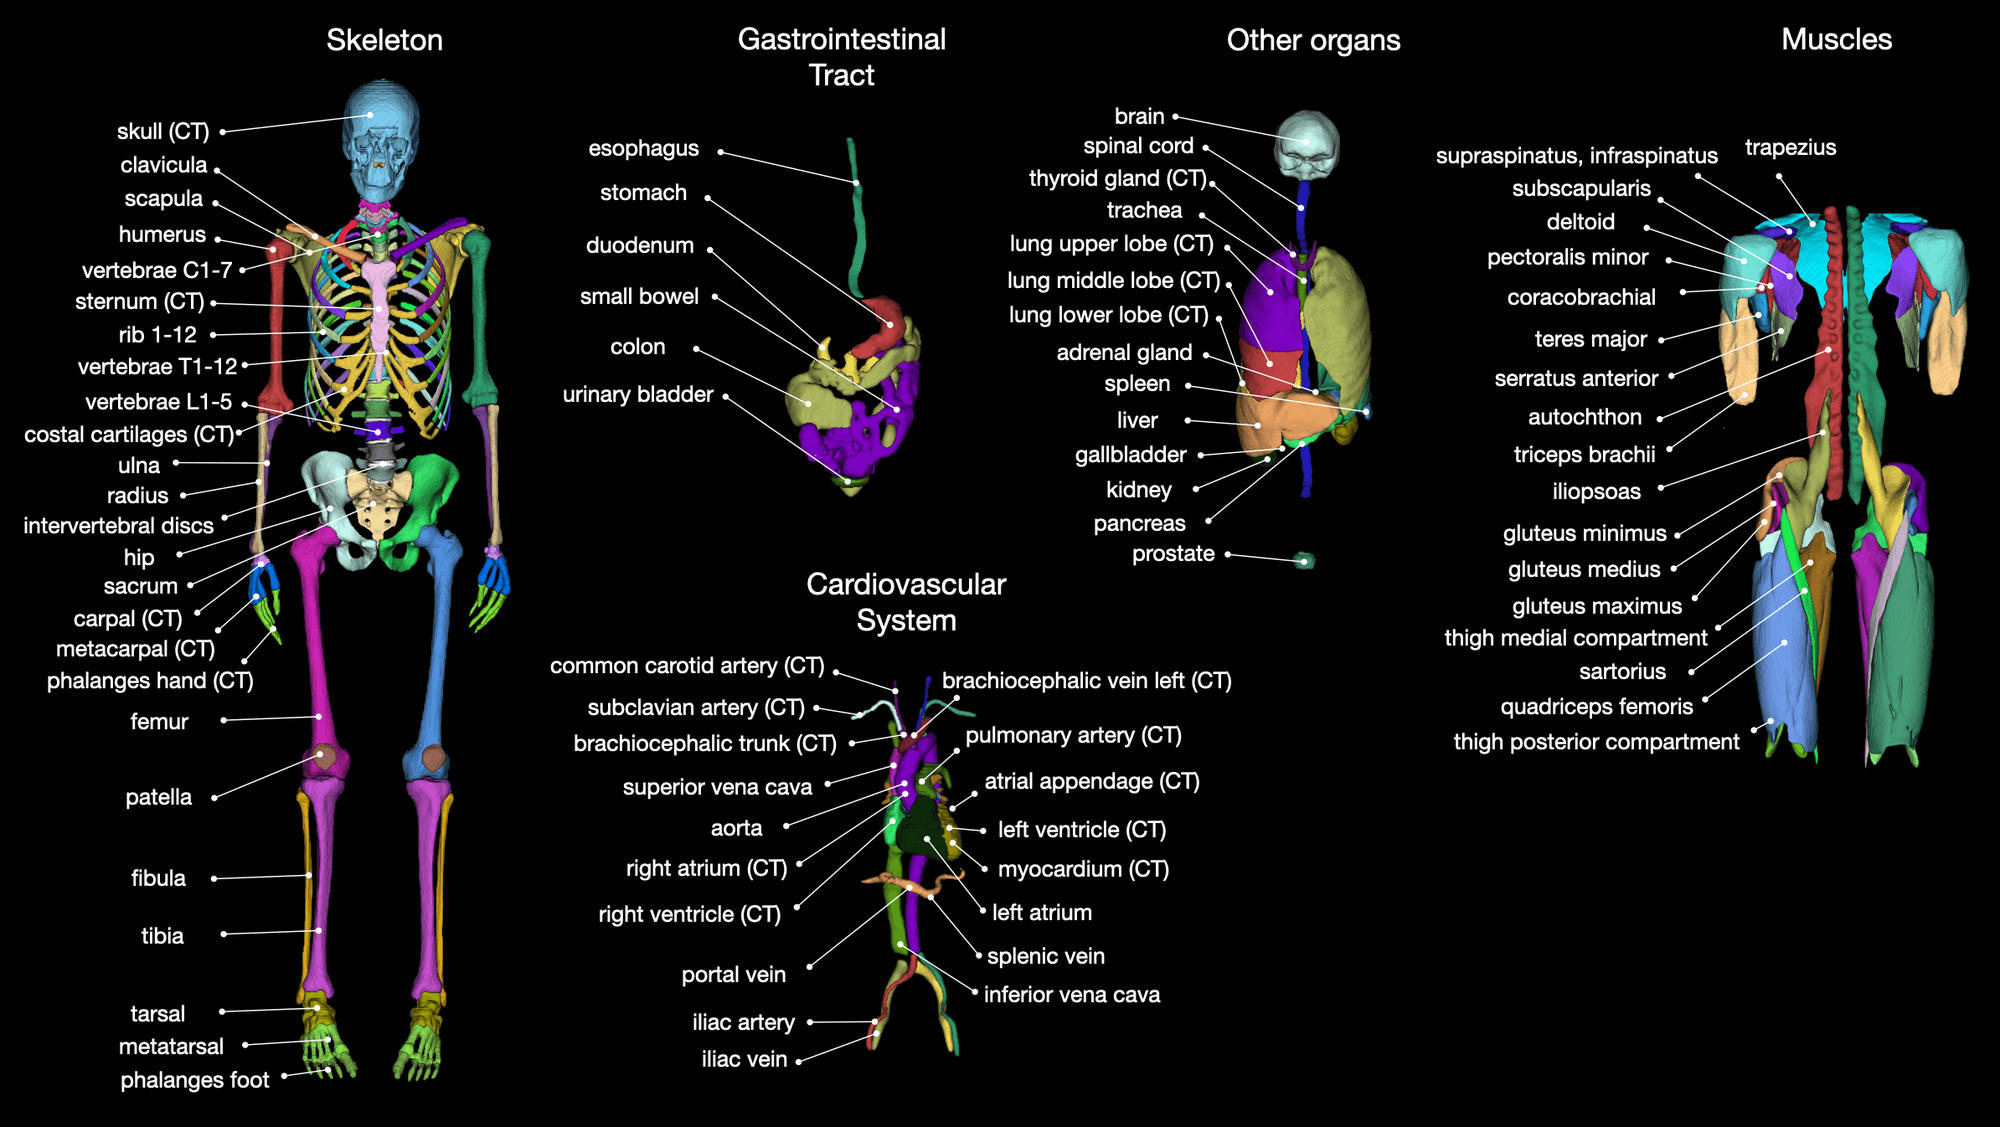
\includegraphics[width=\linewidth,height=0.58\textheight,keepaspectratio]{images/image-restoration-applications/totalsegmentator_overview_classes_v2.png}\\[0.2em]
      {\scriptsize Main CT and MR classes of TotalSegmentator v2. Source: \texttt{TotalSegmentator} repository, \href{https://github.com/wasserth/TotalSegmentator/blob/2af6a1e/resources/imgs/overview_classes_v2.png}{github.com/wasserth/TotalSegmentator} (\texttt{resources/imgs/overview\_classes\_v2.png}, commit 2af6a1e).\par}
  \end{columns}
  {\scriptsize Wasserthal et al., Radiology: Artificial Intelligence 2023, \href{https://arxiv.org/abs/2208.05868v2}{arXiv:2208.05868v2}; Akinci D'Antonoli et al., Radiology 2025, \href{https://arxiv.org/abs/2405.19492v2}{arXiv:2405.19492v2}; repository README.\par}
\end{frame}

\begin{frame}{Promptable and Text-Prompted 3D Segmentation}
  \begin{columns}[T,onlytextwidth]
    \column{0.46\textwidth}
      \begin{itemize}\scriptsize\itemsep0.3em
        \item \textbf{MedSAM} (2024) fine-tuned SAM (covered earlier) on 1,570,263 image-mask pairs from 10 modalities; a box prompt segments one 2D slice at a time.
        \item \textbf{MedSAM2} (2025) fine-tunes SAM2.1-Tiny on over 455,000 3D image-mask pairs and 76,000 video frames. It reads a volume like a video: a box on the middle slice, then SAM~2's memory attention (covered earlier) carries the mask to both ends. Over three annotation rounds, time per CT lesion fell from 525.9\,s by hand to 74.3\,s.
        \item \textbf{nnInteractive} (2025) keeps an nnU-Net ResEnc-L backbone and feeds points, boxes, scribbles or a lasso, drawn on any plane, as extra input channels; the output is a 3D mask. Trained on 64,518 volumes from over 120 datasets; plug-ins for napari, MITK and 3D Slicer.
        \item \textbf{BiomedParse} (2025; 2D, with CT and MRI as slices) prompts with text: one model segments, detects and labels 82 object types in 9 modalities, trained on over 6 million image-mask-description triples.
      \end{itemize}
    \column{0.52\textwidth}
      \centering
      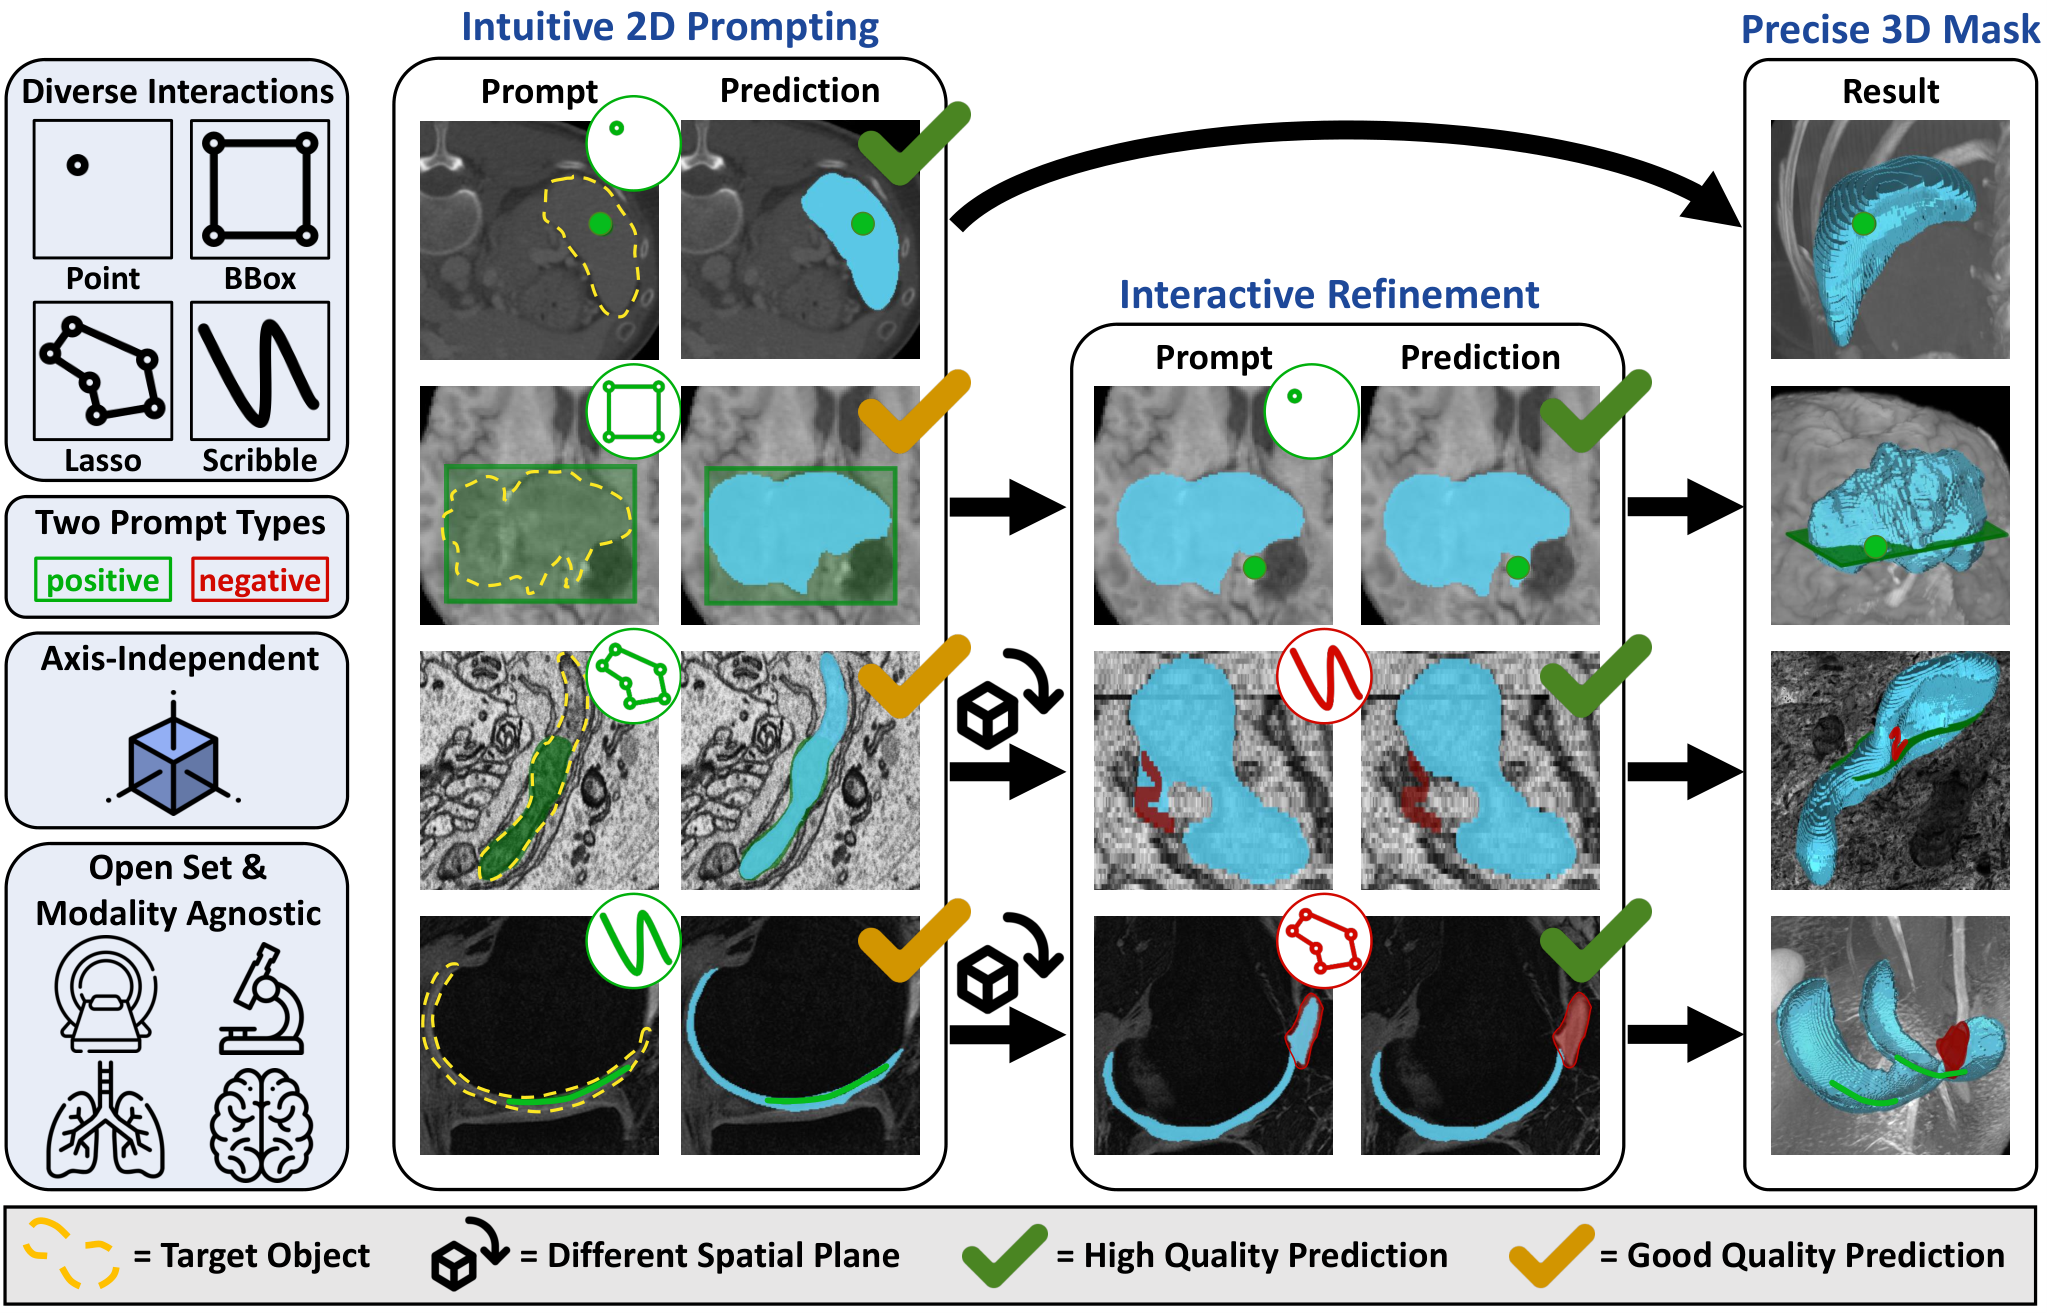
\includegraphics[width=\linewidth,height=0.6\textheight,keepaspectratio]{images/image-restoration-applications/nninteractive_fig1_2d_prompts_to_3d_masks.png}\\[0.2em]
      {\scriptsize Positive or negative 2D prompts on any axis give a 3D mask. Isensee et al., ``nnInteractive: Redefining 3D Promptable Segmentation,'' preprint 2025, \href{https://arxiv.org/abs/2503.08373v1}{arXiv:2503.08373v1}, Figure~1.\par}
  \end{columns}
  {\scriptsize Ma et al., \href{https://arxiv.org/abs/2304.12306v3}{arXiv:2304.12306v3}; Ma et al., ``MedSAM2: Segment Anything in 3D Medical Images and Videos,'' \href{https://arxiv.org/abs/2504.03600v1}{arXiv:2504.03600v1}; Zhao et al., Nature Methods 2025, \href{https://arxiv.org/abs/2405.12971v3}{arXiv:2405.12971v3}.\par}
\end{frame}

\begin{frame}{Pathology: Tile Encoders and Slide-Level MIL}
  \begin{columns}[T,onlytextwidth]
    \column{0.50\textwidth}
      \begin{itemize}\scriptsize\itemsep0.25em
        \item A WSI is cut into tiles and a self-supervised \textbf{tile encoder} embeds each one. Most pathology foundation models reuse DINOv2 (covered earlier) or the related iBOT.
      \end{itemize}
      {\centering\scriptsize
      \begin{tabular}{@{}>{\raggedright\arraybackslash}p{1.5cm} >{\raggedright\arraybackslash}p{1.95cm} >{\raggedright\arraybackslash}p{2.6cm}@{}}
        \toprule
        \textbf{Model} & \textbf{Encoder recipe} & \textbf{Pretraining data} \\
        \midrule
        UNI (2024) & ViT-L, DINOv2 & $>$100M tiles from $>$100k H\&E slides \\
        CONCH (2024) & CoCa (covered earlier) & 1.17M image-caption pairs \\
        Prov-GigaPath (2024) & DINOv2 tiles + LongNet slide encoder & 1.3B tiles from 171,189 slides \\
        Virchow2 (2024) & ViT-H (632M), modified DINOv2 & 3.1M slides \\
        UNI2-h (2025) & ViT-H & $>$200M tiles from $>$350k slides \\
        \bottomrule
      \end{tabular}\par}
    \column{0.48\textwidth}
      \begin{itemize}\scriptsize\itemsep0.3em
        \item \textbf{Multiple-instance learning (MIL)}: a slide has one label (subtype, biomarker) and no tile labels, so it is treated as a bag of $K$ tile embeddings $h_k \in \mathbb{R}^{M}$.
        \item \textbf{Attention pooling} (Ilse et al., 2018):
        \[ z = \sum_{k=1}^{K} a_k h_k, \qquad a_k = \frac{\exp\{w^\top \tanh(V h_k)\}}{\sum_{j=1}^{K}\exp\{w^\top \tanh(V h_j)\}} \]
        $V \in \mathbb{R}^{L\times M}$ and $w \in \mathbb{R}^{L}$ are learned; a classifier reads the slide embedding $z$; the weights $a_k$ map which tiles drove the decision.
        \item Prov-GigaPath instead runs LongNet, a transformer with dilated attention, over the tile sequence, and leads on 25 of its 26 tasks.
      \end{itemize}
  \end{columns}
  {\scriptsize Chen et al. (UNI) and Lu et al. (CONCH), Nature Medicine 2024; Xu et al., Nature 2024; Zimmermann et al., \href{https://arxiv.org/abs/2408.00738v3}{arXiv:2408.00738v3}; \href{https://github.com/mahmoodlab/UNI}{github.com/mahmoodlab/UNI}; Ilse et al., ICML 2018, \href{https://arxiv.org/abs/1802.04712v4}{arXiv:1802.04712v4}, Eq.~7--8.\par}
\end{frame}

\begin{frame}{MedGemma: An Open Medical Vision-Language Model}
  \begin{columns}[T,onlytextwidth]
    \column{0.50\textwidth}
      \begin{itemize}\scriptsize\itemsep0.3em
        \item \textbf{MedGemma} (2025) adapts Google's open Gemma~3 models to medicine. Its encoder, \textbf{MedSigLIP}, is SigLIP-400M tuned on over 33M medical image-text pairs. Sizes: 4B multimodal and 27B.
        \item On MedQA (exam-style questions) MedGemma 4B scores 64.4\% against 50.7\% for Gemma~3 4B. One board-certified thoracic radiologist judged 81\% of its chest X-ray reports to lead to the same or a better clinical decision than the original report.
        \item \textbf{MedGemma 1.5} (2026, 4B) reads a CT or MRI volume as up to 85 axial slices of $896\times896$ pixels (21,760 vision tokens) and a WSI as up to 126 patches; 3D MRI accuracy rose 11 points.
        \item Limits: on MedXpertQA, an out-of-distribution set, MedGemma 27B scores 25.7\% against 54.6\% for o3, a large general-purpose model. The model card: outputs ``are not intended to directly inform clinical diagnosis, patient management decisions, treatment recommendations\ldots''
      \end{itemize}
    \column{0.48\textwidth}
      \centering
      {\scriptsize Open models and what their authors report for local use\par}
      \vspace{0.3em}
      {\scriptsize
      \begin{tabular}{@{}>{\raggedright\arraybackslash}p{2.0cm} >{\raggedright\arraybackslash}p{1.85cm} >{\raggedright\arraybackslash}p{1.95cm}@{}}
        \toprule
        \textbf{Model} & \textbf{Weights licence} & \textbf{Hardware noted} \\
        \midrule
        TotalSegmentator & Apache-2.0 (default tasks) & CPU or GPU \\
        nnU-Net ResEnc M & Apache-2.0 framework & 9.1\,GB VRAM in the 2024 benchmark \\
        nnInteractive & CC BY-NC-SA 4.0 & NVIDIA GPU, 10\,GB recommended \\
        MedSAM2 & CC BY-SA 4.0 tag; card: research and education only & 3D Slicer plug-in; CPU-oriented variant \\
        MedGemma 1.5 4B & Health AI Developer Foundations terms & local GPU inference \\
        \bottomrule
      \end{tabular}\par}
  \end{columns}
  {\scriptsize Sellergren et al., ``MedGemma Technical Report,'' \href{https://arxiv.org/abs/2507.05201v4}{arXiv:2507.05201v4}, Tables~3--4, Figure~4; Sellergren et al., ``MedGemma 1.5 Technical Report,'' \href{https://arxiv.org/abs/2604.05081v2}{arXiv:2604.05081v2}, Section~2.3; \href{https://developers.google.com/health-ai-developer-foundations/medgemma/model-card}{MedGemma 1.5 model card}; licences from each model repository.\par}
\end{frame}

\begin{frame}{Hallucinations and Shortcuts in Medical Imaging}
  \begin{columns}[T,onlytextwidth]
    \column{0.40\textwidth}
      \centering
      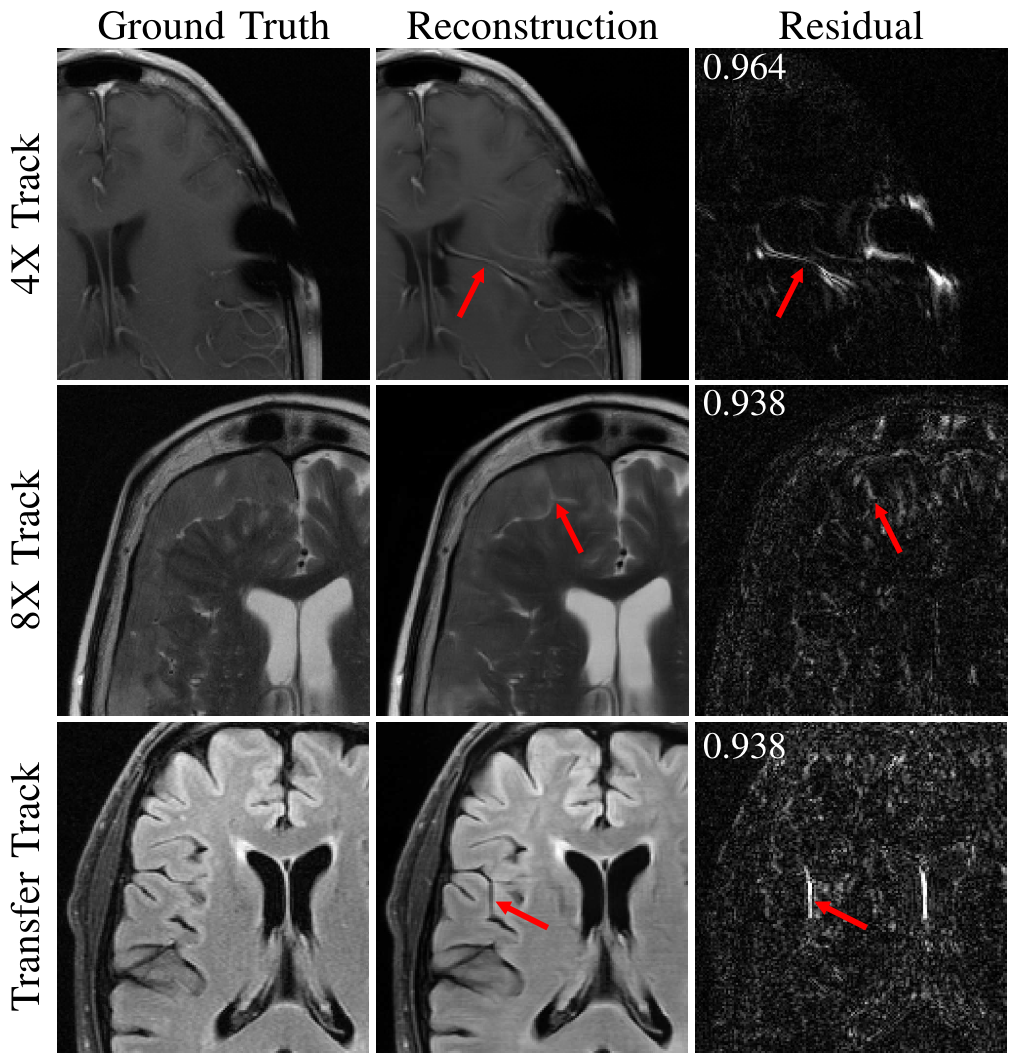
\includegraphics[width=\linewidth,height=0.6\textheight,keepaspectratio]{images/image-restoration-applications/fastmri2020_fig6_reconstruction_hallucinations.png}\\[0.2em]
      {\scriptsize Accelerated brain MRI: reference, learned reconstruction, residual with its SSIM; arrows mark false structures. Muckley et al., ``Results of the 2020 fastMRI Challenge for Machine Learning MR Image Reconstruction,'' IEEE TMI 2021, \href{https://arxiv.org/abs/2012.06318v3}{arXiv:2012.06318v3}, Figure~6.\par}
    \column{0.58\textwidth}
      \begin{itemize}\scriptsize\itemsep0.3em
        \item Learned reconstruction and restoration fill in what the measurements leave open, and the filler comes from the training data. In fastMRI 2020 radiologists found false vessels and sulci; some models ``morphed an abnormality into a more normal brain structure''.
        \item Those images scored SSIM 0.938 to 0.964. The organisers: ``even though these images are considered well-optimized according to this metric, they are not optimized regarding hallucination features.''
        \item The DREAM report defines hallucinations as ``AI-fabricated abnormalities or artifacts that appear visually realistic and highly plausible yet are factually false''. Replacing a real lesion with normal tissue it calls an illusion; both are clinically significant.
        \item \textbf{Shortcut learning}: a chest X-ray pneumothorax classifier reached AUROC 0.87 overall, 0.94 on images with a chest drain and 0.77 without. The drain is the treatment, so the untreated, dangerous cases were common among its false negatives.
        \item Validation practice: report results per subgroup, test on external sites and scanners, and have clinicians read the outputs.
      \end{itemize}
  \end{columns}
  {\scriptsize Xia et al., Journal of Nuclear Medicine 2026, \href{https://arxiv.org/abs/2506.13995v3}{arXiv:2506.13995v3}; Oakden-Rayner et al., ML4H 2019, \href{https://arxiv.org/abs/1909.12475v2}{arXiv:1909.12475v2}, Figure~1(b).\par}
\end{frame}
